% !TEX encoding = UTF-8 Unicode
\documentclass[12pt,english]{article}
\usepackage[utf8]{inputenc}
\usepackage{graphicx}
\usepackage{anysize}
\usepackage{hyperref}
\usepackage{float}
\usepackage{caption}
\marginsize{2cm}{2cm}{1cm}{3cm}
\parskip 2ex
\parindent 0cm
\renewcommand{\contentsname}{Contenidos}
\renewcommand\figurename{Figura}
\title{Práctica 2\\ Acceso al Hardware}
\author{Lluis Ulzurrun De Asanza Sàez\\Victor Grau Moreso \\Mark Antony Holland}
\date{}

\begin{document}

    \maketitle

    \tableofcontents

    \newpage
    
    \section{PersonalData}

    Hemos imprimido todos los valores que nos ofrece el struct de PersonalData. Se puede observar en la \textbf{Figura \ref{s1}} que hemos escogido el color verde para los nombres y el gris para los valores. Hemos observado que en el emulador no\$gba, no están definidos algunos de los valores como el \emph{nombre} y el \emph{mensaje personal} pero en el emulador DeSmuMe si que existen valores para todos.

    \begin{figure}[H] 
    \centering
    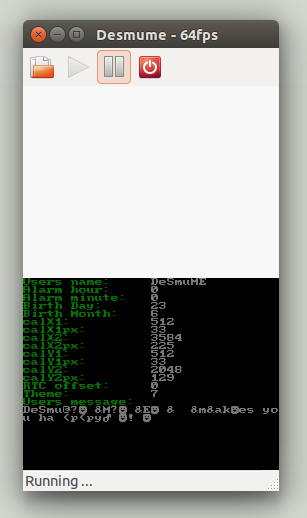
\includegraphics[scale=0.5]{images/personaldata}
    \caption{Captura del programa PersonalData.}
    \label{s1}
    \end{figure}
      
    \newpage
    \section{Paso del tiempo}

    \subsection{stopwatch}

    A continuación están las respuestas de los ejercicios planteados en el boletin.

    \textbf{¿Cual es la definición (prototpipo) de esta función?}
  
    \begin{figure}[H] 
    \centering
    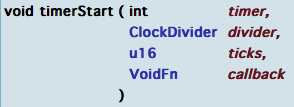
\includegraphics[scale=0.5]{images/timerStart}
    \caption{Prototipo de la función timerStart}
    \end{figure}

    \textbf{Busque también la definición de los argumentos segundo y tercero.}

    ClockDivider\_1024 equivale a dividir el reloj por 1024(~32.7284 kHz) y el 0 como parámetro para el número de ticks antes de desbordar hace que cada tick de nuestro timer equivale a un tick de reloj.

    \subsection{timercallback}

    \textbf{¿Qué significa la función que se le pasa como tercer parámetro?}

    Calcula el valor correcto para el desbordamiento de ticks para una frecuencia dada.

    \textbf{¿Cual es la definición (prototpipo) de la función, el cuarto parámetro, que puede ser llamada por el timer?}

    \texttt{void timerCallBack()}

    \textbf{¿Cómo se le pasa/recoge información a/desde esa función?}

    Con la variable global \emph{play}.

    \newpage
    \subsection{RealTimeClock}

    \textbf{¿Qué dos funciones se utilizan para averiguar la hora y la fecha?}

    Primero llama a \texttt{time} para que devuelve un struct con el unix time, después utiliza gmtime para tratar este \texttt{time\_t} struct y devolver otro struct con el tiempo en un formato más manejable.

    Sus prototipos son las siguientes:

    \texttt{time\_t time(time\_t *t)} y 
    \texttt{struct tm *gmtime(const time\_t *timer)}


    \textbf{¿Cómo inicializa este ejemplo el uso de las dos pantallas de la consola?}

    Con las lineas \#103 y \#106:

    \texttt{lcdMainOnTop();} //del fichero system.h\\
    \texttt{videoSetMode(MODE\_0\_3D);} //del fichero video.h

    \section{Gestión de entrada}

    \subsection{keyboard/keyboard\_async}

    Proporciona un teclado con una consola donde aparece lo que se teclea.

    \begin{figure}[H] 
    \centering
    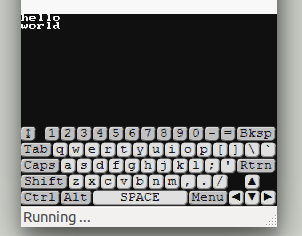
\includegraphics[scale=0.5]{images/keyboard_async}
    \caption{keyboard\_async}
    \end{figure}

    \newpage

    \subsection{keyboard/keyboard\_stdin}

    Lee del teclado como entrada estandard con un tipico program de hola \$(inserta\_nombre).

    \begin{figure}[H] 
    \centering
    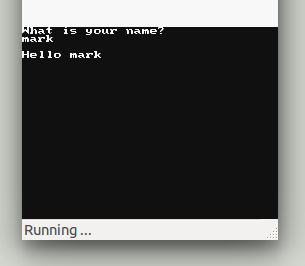
\includegraphics[scale=0.5]{images/keyboard_stdin}
    \caption{keyboard\_stdin}
    \end{figure}

    \subsection{Touch\_Pad/touch\_area/}

    Indice en pantalla que punto de los ejes x/y esta tocando la pantalla el usuario y con que cantidad de fuerza.

    \begin{figure}[H] 
    \centering
    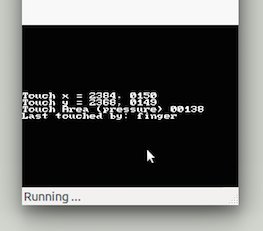
\includegraphics[scale=0.5]{images/touch_area}
    \caption{touch\_area}
    \end{figure}

    \newpage

    \subsection{Touch\_Pad/touch\_look/}

    Proporciona en la pantalla de arriba un mundo 3D donde podemos "mirar" utilizando la pantalla de abajo deslizando el dedo.

    \begin{figure}[H] 
    \centering
    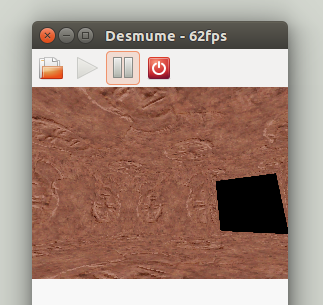
\includegraphics[scale=0.5]{images/touch_look}
    \caption{touch\_look}
    \end{figure}

    \subsection{Touch\_Pad/touch\_test/}

    Parecido al \emph{test\_area} pero proporcionando más información como que botones están siendo pulsados.

    \begin{figure}[H] 
    \centering
    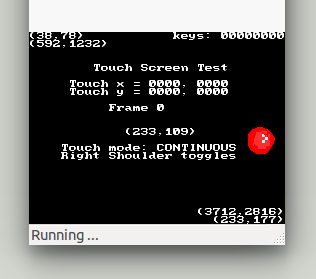
\includegraphics[scale=0.5]{images/touch_test}
    \caption{touch\_test}
    \end{figure}

    \newpage

    \section{Trabajo autónomo}

    Mediante los ejemplos indicados no hubo gran problema para realizar el ejercico, lo único que ha requerido refescar un poco ha sido para mostrar contenido en la pantalla de arriba manteniendo el menu en la de abajo.

    A continuación dejamos capturas del programa mostrando el valor de \texttt{name} y lo mismo trás darle a la función de \texttt{lcdSwap}.

    \begin{figure}[H] 
    \centering
    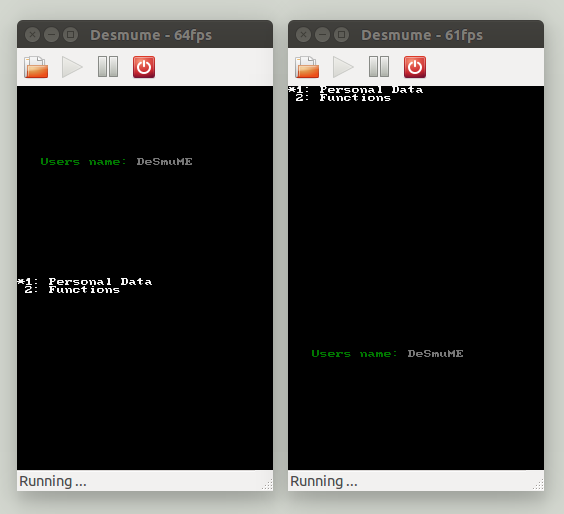
\includegraphics[scale=0.5]{images/prog}
    \caption{Programa con menu}
    \end{figure}

    
\end{document}